\chapter{Materials and Methods}\label{chap:materials-methods}
This chapter introduces the materials and datasets provided in the source paper \citep{Ferber2024}. We then describe how the data were preprocessed and explored, explain how the models were implemented, trained, and evaluated, and finally present the methods used to analyse model explainability.

\section{Data and Materials}\label{sec:method-data-materials}
As part of \citet{Ferber2024}, the authors have published a dataset of 1798 subjects running or walking on a treadmill captured using multi-camera 3D motion capture (\gls{mocapsys}) equipment. The dataset is composed of raw 3d marker data of each \gls{session}, kinematic variables derived from the marker data for each \gls{session} and demographic and antropometric metadata of the subjects. Additionally, the matlab code for the preprocessing of the data, the calculation of the kinematic variables and tutorial notebooks that help ilusatrate how to use their library and read the data from the folder structure are also provided.

\subsection{Measurement protocol}\label{subsec:measurement-protocol}
The complete measurement protocol is described in \citet{Ferber2024}. In this subsection, we provide a summary of the aspects that are most relevant for the methods and analyses presented in this thesis.

The raw marker data was collected using high-speed optoelectronic infrared-based motion capture cameras (MX3/Bonita, Vicon, Oxford, UK) were used to record the position of 9mm spherical retro-reflective markers attached to anatomical landmarks of the subjects at either 120Hz or 200Hz. Depending on the lab, eight or three cameras were used.

\begin{figure}[ht]
    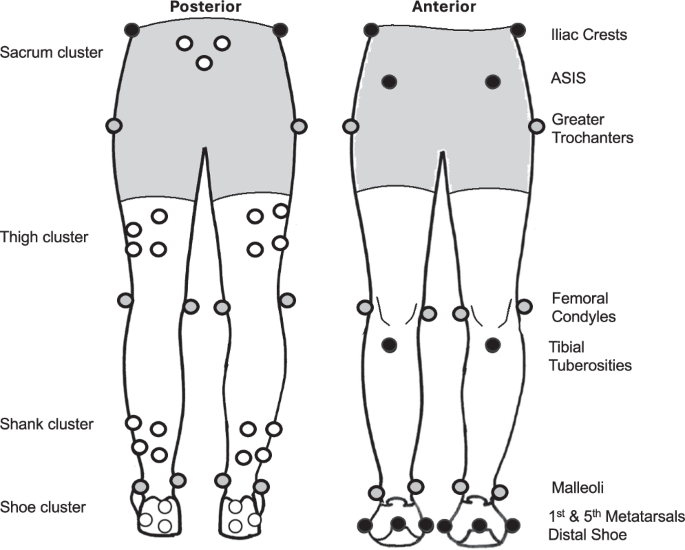
\includegraphics[width=0.5\columnwidth]{images/billateral_marker_position.png}
    \caption{Position of markers on the subjects. Grey markers correspond to core set of markers set, black to additional set and white to the clusters set.}
    \label{fig:marker_position}
\end{figure}

Three sets of markers were used:
\begin{itemize}
    \item Core: Markers attached to the following anatomical landmarks: medial and lateral malleoli, medial and lateral femoral condyles, and greater trochanters.
    \item Additional: Markers attached to the following anatomical landmarks: bilateral 1st and 5th metatarsal heads, distal aspect of the shoe, tibial tuberosity, anterior superior iliac spines, and iliac crests;
    \item Clusters: 3 or 4 markers placed on rigid shells attached to the following anatomical landmarks: sacrum, bilateral thigh and shank, and posterior aspect of both shoes.
\end{itemize}

During the recording of the \glspl{session}{sessions} of all 1798 subjects the 'core' and 'cluster' set of markers were used. The additional set was only used during the recording of the \glspl{session}{sessions} of 1082 subjects. Figure \ref{fig:marker_position} shows the lower body of a subject and the three sets of markers.


\subsection{Dataset Description}\label{subsec:method-dataset-description}
% -- No sessions, provenance, format, variables (angles/velocities per joint and side), available metadata.
% -- Feature description
The source 



\subsection{Code Description}\label{subsec:method-code-description}
-- Matlab code provided by the source paper.
-- My code and repo (high level + refernce to Anex 1)

\subsection{Kinematic Data Extraction}\label{subsec:kinematic-data-extraction}
-- How Kinematic variables are derived.
-- How we obtained angles, anglular velocities from matlab and events...
-- Internal processing assumptions
-- Axis reconstruction
-- Estimations

% TODO: How to integrate EDA and Preprocessing, since it is realted...


\section{Exploratory Data Analysis (EDA)}\label{sec:method-eda}
-- Exploration → Extraction → Preparation, with concrete checks and figures:
-- Tabular data Exploration (sanity and distributions)
-- Dataset inventory (sessions per runner, class prevalence per runner, cycles/session).
-- Missingness map (metadata \& signals); strategy preview (drop/impute).
-- Outliers: per-joint angle/velocity ranges, z-score >3 heatmap by runner (flag sensors/markers).
-- Dimensionality previews: PCA/t-SNE to see separability.


-- Timeseries data Exploration:
-- Visuals: overlay of 20 random stance cycles per class; Markers, Angles, Velocities, ...
-- Analysis of curves
-- Extraction (curve-level descriptors)


-- Preparation (decisions fixed before modelling)

-- Group-aware split policy (runner-level), ensuring no cycle leakage across folds.
-- Class-imbalance diagnostics (AUC-PR baseline, per-runner prevalence plots).
-- Filtering rules for cycles/sessions (min cycles per session, quality thresholds).

-- Final feature set(s) to carry forward (e.g., summaries, PC scores, raw curves for DL)

% TODO: Maybe we keep outliers and filering here?


\section{Pre-processing}\label{sec:method-preprocessing}
-- Tabular:
    -- filtering, subject identification, outliers, cleaning, etc..
    -- Final dataset creation -> Give name to track

-- Timeseries:
    -- Extraction of angles and angular velocities as mentioned in literature.
    -- Extraction of events
    -- Combination of events and TS
    -- Cycle Segmentation and normalization -> Reference papers either here or in SOTA.

\subsection{Feature Engineering}\label{subsec:method-feature-engineering}
-- Transformations and feature extraction
    -- Dominant Leg -> VIF reduction
    -- Obtaining a representative curve
        -- Curve registration attempt and Actual result

-- Feature selection:
    -- MRMR for feature selection

\subsection{Feature Selection}\label{subsec:method-feature-selection}
-- Transformations and feature extraction
    -- Dominant Leg -> VIF reduction
    -- Obtaining a representative curve
        -- Curve registration attempt and Actual result

-- Feature selection:
    -- MRMR for feature selection

% \subsection{Tabular Data}\label{subsec:method-tabular-data}
% -- Correlations mutual information, ...
% -- Collinearity: PCA, VIF, ...
% -- Left-right features - Dominant leg extraction
% -- Collinearity reduction

% \subsection{Timeseries Data}\label{subsec:method-timeseries-data}
% -- Segmentation: TD/TO, stance, swing, ...
% -- Normalisation/standardisation

\subsection{Final Feature Sets}\label{subsec:method-final-feature-sets}
-- Summary of the feature by dataset.

\section{Models}\label{sec:method-models}
\subsection{Baseline (Tabular)}\label{subsec:method-baselines}
\subsection{Deep Learning}\label{subsec:method-deep-learning}
-- Unilateral LSTM
-- Bilateral LSTM
-- Multimodal
-- TMAG
-- MC DCNN

-- Add special tuning for class imbalance, etc...
-- Architecture choices (hyperparameters, etc...)
-- class imbalance, oversampling, etc... TBD Where to put this? -> Explain in the models that used it. We will give results for each option individually.

\section{Evaluation Protocol}\label{sec:method-evaluation-protocol}
-- The blueprint before we run anything.
-- Questions/Hipothesis, grouping, leakage, validation scheme (group-aware train/val/test)
-- Evaluation protocol -> Measurements, statistics. How are we scoring the experimentriment. (Primary, Secondary metric, Threshold rule, ...).
-- Significance Tests. How do we know something is "Better" (DeLong's test)?
-- CI 95 \%
-- Research questions (RQs), validation scheme (group-aware train/val/test), splits, primary/secondary metrics.
-- Justify the choices , but do not present any results yet...

\subsection{Evaluation Metrics}\label{subsec:method-evaluation-metrics}
- AUC ROC + PR for class imbalance + Macro F1 score for threshold.

\subsection{Training and Validation Strategy}\label{subsec:method-training-validation-strategy}
-- Train, test, validation split.
-- Group-aware split policy (runner-level), ensuring no cycle leakage across folds.
-- Class-imbalance diagnostics (AUC-PR baseline, prevalence).

\subsection{Hyperparameter Tuning}\label{subsec:method-hyperparameter-tuning}
-- Grid search, random search, ...
-- Cross-validation, nested cross-validation, ...
-- Early stopping, ...
-- Hyperparameter tuning strategy.


\section{Explainability}\label{sec:method-explainability}
<Draft> This project would have been set up differently if the sole goal had been to build and deploy an injury detection model. In that case, explainability would mostly be used just to debug the model, and the focus would shift toward making data collection easier, choosing an efficient architecture, and reducing resource use. In our case, though, explainability is central: a deep learning model with an AUC-ROC of 0.7 doesn't add much value if it remains a black box.

To get the most out of this work, we used both intrinsic methods and Explainable AI (XAI) techniques, as in \cite{FuentesJimnez2025}, to make the model's decisions more transparent.

\subsection{Intrinsic Explainability}\label{subsec:method-intrinsic-explainability}
- Random Forest, linear regression, etc...
-- Pros, Cons, etc..
-- what affects them?

\subsection{Post-hoc Explainability}\label{subsec:method-posthoc-explainability}
-- SHAPs, Saliency maps, feature permutation?



% \section{Reproducibility Assets}\label{sec:method-reproducibility}
% -- code repository structure, libraries, etc...
